%! TEX root = ../thesis.tex
\section{The European Law-Making Process}
\label{sec:background}

\subsection{Representative Democracies}

In representative democracies, citizens elect politicians to represent them in the various branches of the government.
The executive branch is in charge of executing and enforcing the laws.
Representatives of the executive branch can also propose new laws, but, to avoid a concentration of power, they cannot pass new legislation without the approval of the legislative branch.
The legislative branch, typically a parliament, represents both the people and the sub-governmental entities (such as states and municipalities).
Parliamentarians  can propose new legislation or amend propositions made by the executive branch.
Finally, the judicial branch balances the power of the executive branch and the legislative branch through its ability to decide whether the laws are constitutional.

Here, we focus on the European Union (EU).
The EU is a political and economic union of 28 countries called member states.
This union enables them to share their markets, to ease mobility across borders, to favor economic development, and to harmonize laws.
The EU covers an estimated population of 513 million, and up to 84\% of member states' national laws emanate from the EU \cite{miller2010much}.
Hence, EU laws have a significant impact on the life of many people.
European institutions make efforts to be transparent.
They make a lot of valuable data available online: parliamentary amendments, meetings by the commissioners with civil society, and a transparency register to monitor interest groups.
%These efforts give access to large datasets of great value.

The EU political system is broadly similar to that of a regular state.
The 751 parliament representatives (MEPs, for Member of the European Parliament) are elected every five years by universal suffrage.
The executive branch is called the \textit{European Commission}.
The legislative branch consists of the \textit{European Parliament} and of the \textit{Council of Ministers}.
The Parliament is divided into 20 committees, comprising sub-sets of MEPs and specialized in some particular policy area (such as fisheries, judiciary affairs, transportation, and trade).
Each MEP is a member of at least one committee.
The myriad of national parties aggregate into a small number of political groups.

\subsection{The Ordinary Legislative Procedure}

We now describe the EU law-making process in some detail, leading up to our modeling assumptions.
Under the Treaty of Lisbon \cite{eu2007lisbon}, which marks the beginning of the 7\th legislature in 2009, the Parliament's powers were increased.
The Parliament became central in the process through which new laws are created.
This process can take the form of various procedures, the main one being the \textit{ordinary legislative procedure} (OLP)~\cite{europarl2018ordinary}.
Through the OLP, the Commission initiates a legislative proposal, and the Parliament must adopt it in order for the proposal to become a law.
Other procedures exist, where the Parliament is not necessarily involved.
Since 2009, the Parliament has dealt with 90\% of all new laws via the OLP.
In this regard, we focus on the dynamics of the legislative process in the Parliament.
A sketch of the OLP is illustrated in Figure~\ref{fig:ols} and described in the next paragraphs.

\begin{figure}
  \centering
	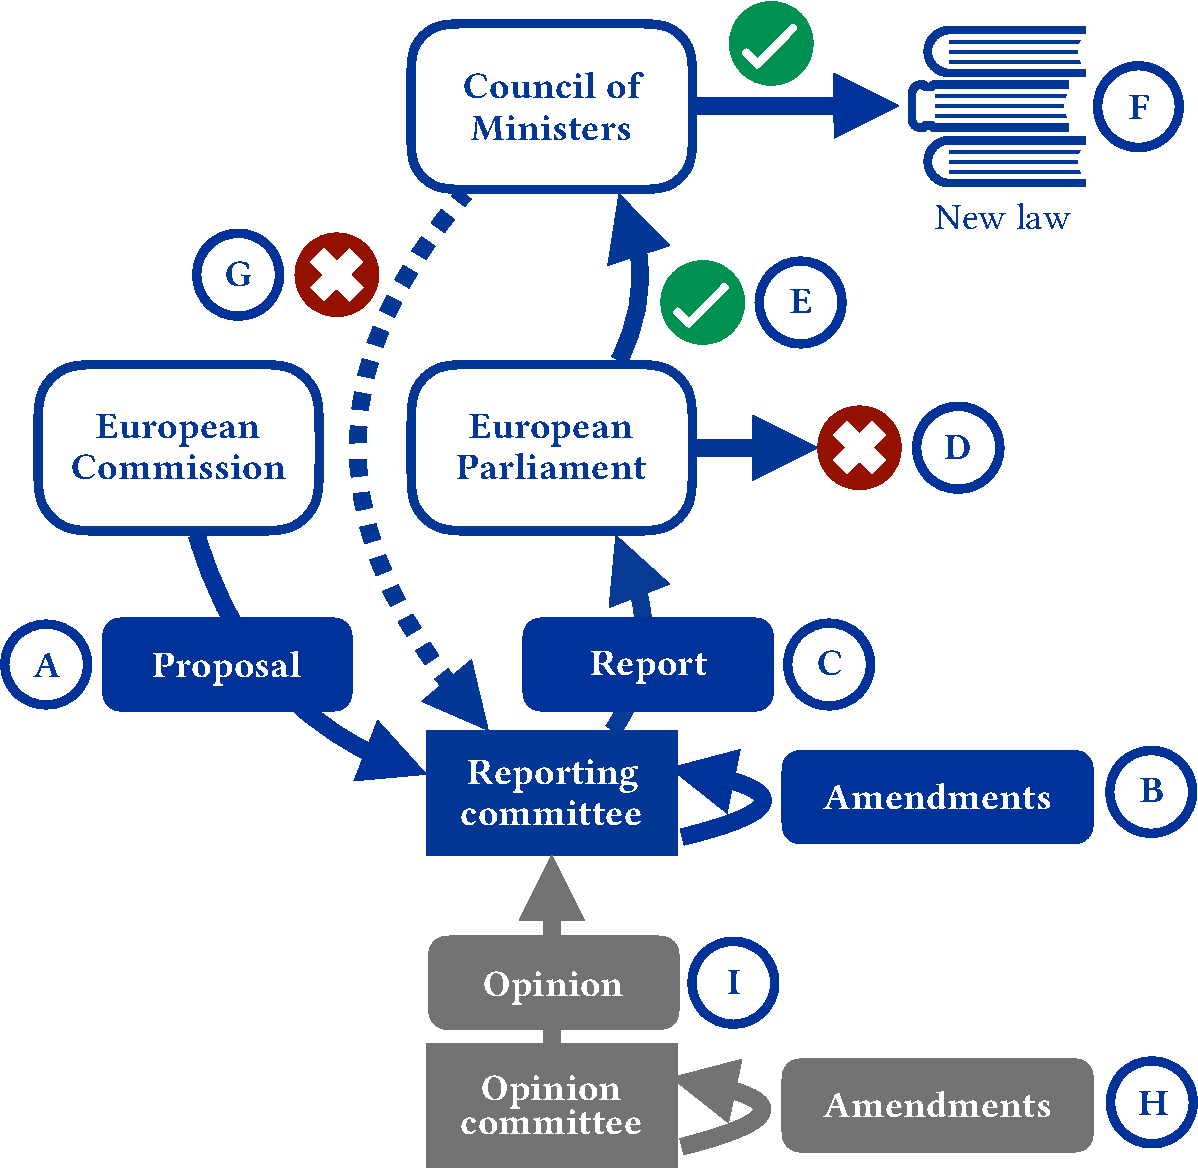
\includegraphics[width=\linewidth*2/3]{lmp-ols}
	\caption{
		Sketch of the \textit{ordinary legislative procedure}.
		(A) The Commission submits a legislative proposal to one of the Parliament committees.
		(B) The proposal is amended and (C) submitted to vote to the whole Parliament.
		(D) If it is rejected, the proposal is abandoned.
		(E) If it is accepted, it is transferred to the Council.
		(F) If the Council accepts the amended proposal, a new law is adopted.
		(G) If the Council amends it, it is sent back to the committee.
		(H) Other committees can optionally make amendments and (I) suggest them to the reporting committee.
	}
	\label{fig:ols}
\end{figure}

To create a new law, (A) the Commission drafts a legislative \textit{proposal} and transfers it to the corresponding committee of the Parliament.
For instance, if the proposal introduces regulations on greenhouse-gas emissions, it is transferred to the Environment Committee.
The committee appoints a \textit{rapporteur} to lead the debate.
The role of the committee is to write a \textit{report} in the form of \textit{amendments} to the proposal, i.e., insertions in or deletions of parts of the proposal.
The rapporteur first seeks external expertise to draft a report.
Then, (B) other MEPs on the committee can in turn propose amendments to the proposal.
To constitute the final report to be submitted to the whole Parliament, each amendment by the rapporteur or by other MEPs is therefore voted on within the committee.
Once the committee finds a consensus, (C) they transfer the report to the whole Parliament.

In the plenary session, the Parliament holds a vote on the report.
(D) If rejected, the proposal is abandoned; (E) if accepted, the report, establishing the Parliament's position on the proposal, is transferred to the Council of Ministers.
The report is therefore an important document and the rapporteur has an important role to play.
The ministers (of the different EU countries) can accept the report, (F) in which case, the proposal is adopted with the Parliament's amendments and a new law is created; or they can make amendments, (G) in which case it is transferred back to the parliamentary committee.
At this stage, we say that a law has gone through the first \textit{reading}.

Other committees can also independently decide to address an \textit{opinion} to the reporting committee.
For instance, the Transportation Committee might consider that it is also concerned by greenhouse-gas emissions and that it is entitled to give its opinion to the Environment Committee.
An opinion is similar to a report in that it contains amendments to the proposal.
It is created similarly to a report, i.e., (H) the opinion committee appoints a rapporteur to draft an opinion, and other MEPs can propose amendments.
(I) The opinion committee then transfers its opinion to the reporting committee.
An opinion differs from a report in that it is not voted by the whole Parliament (only the report is), and the reporting committee is free to take into account the amendments from the opinion.
Amendments from the opinion committee can, however, be in conflict with amendments from the reporting committee, and MEPs from the reporting committee will also have to vote on those.
We refer to reports and opinions as \textit{dossiers}.

This iterative process can be repeated up to three times (three readings).
The third reading, called conciliation, involves a negotiation between the Parliament and the Council.
During the 8\th legislature for example, 99\% of all laws were adopted after the first reading, i.e., after amendments made by both the Parliament and the Council, and 89\% were adopted directly after amendments by the Parliament, i.e., the Council accepted it without making amendments.

